\documentclass{article}
% \usepackage[headsepline]{scrlayer-scrpage}

% \ihead{Levin}
% \ohead{\thepage}
% \pagestyle{scrheadings}
\usepackage{bbm}
\usepackage{amsmath,amsfonts,amsthm,amssymb,amsopn,bm}
\usepackage[margin=.9in]{geometry}
\usepackage{graphicx}
\usepackage{url}
\usepackage[usenames,dvipsnames]{color}
\usepackage{fancyhdr}
\usepackage{multirow}
\usepackage{pythonhighlight}
\usepackage{pgfplots}

\usepackage{minted}
% Default fixed font does not support bold face
\DeclareFixedFont{\ttb}{T1}{txtt}{bx}{n}{12} % for bold
\DeclareFixedFont{\ttm}{T1}{txtt}{m}{n}{12}  % for normal

% Custom colors
\usepackage{color}
\definecolor{deepblue}{rgb}{0,0,0.5}
\definecolor{deepred}{rgb}{0.6,0,0}
\definecolor{deepgreen}{rgb}{0,0.5,0}

\usepackage{listings}

% Python style for highlighting
\newcommand\pythonstyle{\lstset{
language=Python,
basicstyle=\ttm,
otherkeywords={self},             % Add keywords here
keywordstyle=\ttb\color{deepblue},
emph={MyClass,__init__},          % Custom highlighting
emphstyle=\ttb\color{deepred},    % Custom highlighting style
stringstyle=\color{deepgreen},
frame=tb,                         % Any extra options here
showstringspaces=false            % 
}}


% Python environment
\lstnewenvironment{python}[1][]
{
\pythonstyle
\lstset{#1}
}
{}

% Python for external files
\newcommand\pythonexternal[2][]{{
\pythonstyle
\lstinputlisting[#1]{#2}}}

% Python for inline
\newcommand\pythoninline[1]{{\pythonstyle\lstinline!#1!}}

% Some additional tweaking for this package can be made in the preamble. To change the size of each plot and also guarantee backwards compatibility (recommended) add the next line:

\pgfplotsset{width=10cm,compat=1.9}

% This changes the size of each pgfplot figure to 10 centimeters, which is huge; you may use different units (pt, mm, in). The compat parameter is for the code to work on the package version 1.9 or later.

% Since LaTeX was not initially conceived with plotting capabilities in mind, when there are several pgfplot figures in your document or they are very complex, it takes a considerable amount of time to render them. To improve the compiling time you can configure the package to export the figures to separate PDF files and then import them into the document, add the code shown below to the preamble:

\usepgfplotslibrary{external}

\tikzexternalize 

\newcommand{\field}[1]{\mathbb{#1}}
\newcommand{\1}{\mathbf{1}}
\newcommand{\I}{\mathbbm{1}}
\newcommand{\E}{\mathbb{E}} 
\newcommand{\V}{\mathbb{V}} 
\renewcommand{\P}{\mathbb{P}}
 \newcommand{\ind}{\perp\!\!\!\perp}
 \DeclareMathOperator{\rank}{rank}
\newcommand{\R}{\field{R}} % real domain
% \newcommand{\C}{\field{C}} % complex domain
\newcommand{\F}{\field{F}} % functional domain

\newcommand{\T}{^{\textrm T}} % transpose

\def\diag{\text{diag}}

%% operator in linear algebra, functional analysis
\newcommand{\inner}[2]{#1\cdot #2}
\newcommand{\norm}[1]{\left\|#1\right\|}
\newcommand{\twonorm}[1]{\|#1\|_2^2}
% operator in functios, maps such as M: domain1 --> domain 2
\newcommand{\Map}[1]{\mathcal{#1}}
\renewcommand{\theenumi}{\alph{enumi}} 

\newcommand{\Perp}{\perp \! \! \! \perp}

\newcommand\independent{\protect\mathpalette{\protect\independenT}{\perp}}
\def\independenT#1#2{\mathrel{\rlap{$#1#2$}\mkern2mu{#1#2}}}
\newcommand{\vct}[1]{\boldsymbol{#1}} % vector
\newcommand{\mat}[1]{\boldsymbol{#1}} % matrix
\newcommand{\cst}[1]{\mathsf{#1}} % constant
\newcommand{\ProbOpr}[1]{\mathbb{#1}}
\newcommand{\points}[1]{\small\textcolor{magenta}{\emph{[#1 points]}} \normalsize}
\date{{}}

\setlength\parindent{0px}

\begin{document}
\title{Homework \#1}
\author{\normalsize{Spring 2020, CSE 546: Machine Learning}\\
\normalsize{\bf Roman Levin} \\
\normalsize{\bf 1721898} \\
}
\maketitle
Collaborators: compared answers with Tyler Chen, Diya Sashidhar, Katherine Owens
\section*{Problems A}
\subsection*{Conceptual Questions}
\noindent\rule{\textwidth}{1pt}

A.0 {\bf Solution:}\\
\begin{itemize}
    \item {\bf Bias} -- how far our expected model is from the best possible estimator. Or, in expectation (over all possible data), how well our model fits the best possible estimator.\\
    \\
    {\bf Variance} -- how much on average our model changes (how much the predictions vary) around our expected model over iid resampling of the data from the underlying generating distribution. (That is, every time we draw a new dataset from the underlying distribution and refit the model.) \\
    \\
    {\bf Bias-Variance Tradeoff} -- The true total expected error of our model decomposes into irreducible error and learning error. The learning error decomposes into the bias squared and variance squared. So, we could reduce the learning error by reducing the bias and/or the variance of our model. However, usually models with lower bias have higher variance and vice versa, so there is a tradeoff between bias and variance. We would like to find the sweet spot, that is, we want to balance bias and variance to get smaller learning error.
    \item As the model {\bf complexity increases, bias decreases and variance increases}. As the model {\bf complexity decreases, bias increases and variance decreases}.
    \item {\bf False}
    \item {\bf True} (Or True-ish. Usually, using more data has a regularizing effect, so more data reduces variance, especially if the model is expressive enough to capture the "truth". However, we could also think of artificial counter-examples like a model which has no trainable parameters and just outputs 42 for any input. For this model, the variance will be always zero, but we would probably prefer models with trainable parameters.)
    \item {\bf False} (e.g. using zero features does not result in better models)
    \item {\bf Train set} (we should NEVER use the test set for tuning the model)
    \item {\bf False}
\end{itemize}

\noindent\rule{\textwidth}{1pt}
\subsection*{MLE}
\noindent\rule{\textwidth}{1pt}
A.1 {\bf Solution:}\\
\begin{enumerate}
    \item Let's find the ML estimator for an arbitrary n: $\lambda_{MLE} = \arg\min_\lambda L(\lambda)$.
    \begin{itemize}
        \item $L(\lambda) = -\log \prod_{i=1}^n \mathrm{Poi}(x_i|\lambda) =  -\sum_{i=1}^n (-\lambda +  x_i\log \lambda - \log x_i!)$
        \item $L'(\lambda) = n - \sum_i x_i/\lambda = 0 \Leftrightarrow \boxed{\lambda_{MLE} = \frac{\sum_{i=1}^n x_i}{n}}$
        \item (Check $L''(\lambda) = \sum_i x_i/\lambda^2 \ge 0$ since $x_i \ge 0$. But if at least one of $x_i > 0$, then $L''(\lambda) > 0$, so we indeed found the minimum. If $\forall x_i = 0$, then $\lambda_{MLE} = 0$ which is also consistent with the formula above. $\Box$
        \\
        The answer for part a. is then: $$\boxed{\lambda_{MLE} = \frac{\sum_{i=1}^5 x_i}{5} = 6/5}$$
    \end{itemize}
    \item $$\boxed{\lambda_{MLE} = \frac{\sum_{i=1}^6 x_i}{6} = 10/6 = 5/3}$$
    \item $$\boxed{\lambda_{MLE, 5} = 6/5, \; \; \lambda_{MLE, 6} = 5/3}$$
    
\end{enumerate}

\noindent\rule{\textwidth}{1pt}

\noindent\rule{\textwidth}{1pt}
A.2 {\bf Solution:}\\
Notation: $\I{\{\cdot\}}$ stands for an indicator function.\\
\begin{itemize}
    \item The likelihood: $L(\theta) = \prod_{i=1}^n \frac{1}{\theta}\I{\{ x_i \in [0,\theta]\}}$. We want to find $\theta_{MLE}$ which maximizes $L(\theta).$
    \item Note that $\exists x_i \not \in [0,\theta] \Rightarrow L(\theta)$, otherwise $L(\theta) = \frac{1}{\theta^n} > 0$ since $\theta \ge 0$. Note also that decreasing $\theta$ increases $\frac{1}{\theta^n}$. So we need to choose the smallest possible $\theta$, s.t. $\forall i: x_i \in [0,\theta]$.
    \item The smallest possible $\theta$, s.t. $\forall i: x_i \in [0,\theta]$ is $$
    \boxed{ \theta_{MLE} = \max_i x_i }$$
\end{itemize}
\noindent\rule{\textwidth}{1pt}
\subsection*{Overfitting}
\noindent\rule{\textwidth}{1pt}
\\
% Suppose we have \( N \) labeled samples \( S = \{ (x_i,y_i) \}_{i=1}^{n} \) drawn i.i.d. from an underlying distribution \( \mathcal{D} \).
%     Suppose we decide to break this sent into a set \( S_{\text{train}} \) of size \( N_{\text{train}} \) and a set \( S_{\text{test}} \) of size \( N_{\text{test}} \) samples for our training and test set, so \( N = N_{\text{train}} + N_{\text{test}} \), and \( S = S_{\text{train}} \cup S_{\text{test}} \).
%     Recall the definition of the true least squares error of \( f \):
%     \begin{align*}
%         \epsilon(f) = \EE_{(x,y)\sim\mathcal{D}}[ (f(x) - y)^2 ],
%     \end{align*}
%     where the subscript \( (x,y) \sim \mathcal{D} \) makes clear that our input-output pairs are sampled according to \( \mathcal{D} \).
%     Our training and test losses are defined as:
%     \begin{align*}
%         \widehat\epsilon_{\text{train}}(f) 
%         &= \frac{1}{N_{\text{train}}} \sum_{(x,y)\in S_{\text{train}}} (f(x)-y)^2
%         \\
%         \widehat\epsilon_{\text{test}}(f) 
%         &= \frac{1}{N_{\text{test}}} \sum_{(x,y)\in S_{\text{train}}} (f(x)-y)^2
%     \end{align*}
%     We then train our algorithm (for example, using linear least squares regression) using the training set to obtain \( \widehat{f} \).
%     \begin{enumerate}
%         \item (bias: the test error) For all fixed \( f \) (before we've seen any data) show that
%             \begin{align*}
%                 \EE_{\text{train}}[ \widehat\epsilon_{\text{train}}(f) ] 
%                 = \EE_{\text{test}}[ \widehat\epsilon_{\text{test}}(f)]
%                 = \epsilon(f).
%             \end{align*}
%             Use a similar line of reasoning to show that the test error is an unbiased estimate of our true error for \( \widehat{f} \).
%             Specifically, show that:
%             \begin{align*}
%                 \EE_{\text{test}}[ \widehat\epsilon_{\text{test}}(\widehat{f}) ]
%                 = \epsilon(\widehat{f}).
%             \end{align*}
%         \item (bias: the train/dev error)
%             Is the above equation true (in general) with regards to the training loss? 
%             Specifically, does \( \EE_{\text{train}}[ \widehat\epsilon_{\text{train}}(\widehat{f}) ] \) equal \( \EE_{\text{train}}[\epsilon(\widehat{f})] \)? 
%             If so, why? 
%             If not, give a clear argument as to where your previous argument breaks down. 
%         \item Let \( \mathcal{F} = (f_1,f_2, \ldots) \) be a collection of functions and let \( \widehat{f}_{\text{train}} \) minimize the training error such that \( \widehat\epsilon_{\text{train}}(\widehat{f}_{\text{train}}) \leq \widehat\epsilon_{\text{train}}(f) \) for all \( f\in\mathcal{F} \).
%             Show that,
%             \begin{align*}
%                 \EE_{\text{train}}[ \widehat\epsilon_{\text{train}}(\widehat{f}_{\text{train}}) ] 
%                 \leq \EE_{\text{test}}[ \widehat\epsilon_{\text{test}}(\widehat{f}_{\text{test}}) ] 
%             \end{align*}
%             (Hint: note that,
%             \begin{align*}
%                 \EE_{\text{train,train}}[ \widehat\epsilon_{\text{test}}(\widehat{f}_{\text{train}}) ] 
%                 &= \sum_{f\in\mathcal{F}} \EE_{\text{train,test}}[ \widehat\epsilon_{\text{test}}(f) \bOne\{ \widehat{f}_{\text{train}} = f \} ]
%                 \\&= \sum_{f\in\mathcal{F}} \EE_{\text{test}}[ \widehat\epsilon_{\text{test}}(f)] \EE_{\text{train}}[\bOne\{ \widehat{f}_{\text{train}} = f \} ]
%                 \\&= \sum_{f\in\mathcal{F}} \EE_{\text{test}}[ \widehat\epsilon_{\text{test}}(f)] \PP_{\text{train}}[\widehat{f}_{\text{train}} = f ]
%             \end{align*}
%             where the second equality follows from the independence between the train and test set.)
%     \end{enumerate}
% \\
A.3 {\bf Solution:}\\
\begin{enumerate}
    \item \begin{align*}
                \E_{\text{train}}[ \widehat\epsilon_{\text{train}}(f) ]
        &= \E_{\text{train}}\left[\frac{1}{N_{\text{train}}} \sum_{(x,y)\in S_{\text{train}}} (f(x)-y)^2\right] = 
        \frac{1}{N_{\text{train}}} \E_{\text{train}}\left[\sum_{(x,y)\in S_{\text{train}}} (f(x)-y)^2\right]  \\
        &= \frac{1}{N_{\text{train}}} N_{\text{train}} \E_{(x,y)\sim\mathcal{D}}[ (f(x) - y)^2 ] =  \E_{(x,y)\sim\mathcal{D}}[ (f(x) - y)^2 ] = \epsilon(f) \qquad \Box
        \end{align*}
        Where the third equality follows from the fact that the points in $S_{\text{train}}$ are iid, and that sampling the entire $S_{\text{train}}$ iid and picking the points from it one by one is equivalent to just sampling one point from the generating distribution over and over again $N_{\text{train}}$ times (provided that $f$ is independent of $S_{\text{train}}$, because otherwise we cannot assume that $(f(x) - y)^2$ are iid in $\sum_{(x,y)\in S_{\text{train}}} (f(x)-y)^2)$. $f$ is indeed independent of the training set by the problem statement). 
        \begin{align*}
        \E_{\text{test}}[ \widehat\epsilon_{\text{test}}(f) ]
        &= \E_{\text{test}}\left[\frac{1}{N_{\text{test}}} \sum_{(x,y)\in S_{\text{test}}} (f(x)-y)^2\right] = 
        \frac{1}{N_{\text{test}}} \E_{\text{test}}\left[\sum_{(x,y)\in S_{\text{test}}} (f(x)-y)^2\right]  \\
        &= \frac{1}{N_{\text{test}}} N_{\text{test}} \E_{(x,y)\sim\mathcal{D}}[ (f(x) - y)^2 ] =  \E_{(x,y)\sim\mathcal{D}}[ (f(x) - y)^2 ] = \epsilon(f)\qquad \Box
        \end{align*}
        Where the third equality follows from the fact that the points in $S_{\text{test}}$ are iid, and that sampling the entire $S_{\text{test}}$ iid and picking the points from it one by one is equivalent to just sampling one point from the generating distribution over and over again $N_{\text{test}}$ times (provided that $f$ is independent of $S_{\text{test}}$, because otherwise we cannot assume that $(f(x) - y)^2$ are iid in $\sum_{(x,y)\in S_{\text{test}}} (f(x)-y)^2)$. $f$ is indeed independent of the test set by the problem statement).
        \begin{align*}
        \E_{\text{test}}[ \widehat\epsilon_{\text{test}}(\widehat{f}) ]
        &= \E_{\text{test}}\left[\frac{1}{N_{\text{test}}} \sum_{(x,y)\in S_{\text{test}}} (\widehat{f}(x)-y)^2\right] = 
        \frac{1}{N_{\text{test}}} \E_{\text{test}}\left[\sum_{(x,y)\in S_{\text{test}}} (\widehat{f}(x)-y)^2\right]  \\
        &= \frac{1}{N_{\text{test}}} N_{\text{test}} \E_{(x,y)\sim\mathcal{D}}[ (\widehat{f}(x) - y)^2 ] =  \E_{(x,y)\sim\mathcal{D}}[ (\widehat{f}(x) - y)^2 ] = \epsilon(\widehat{f})\qquad \Box
        \end{align*}
        Where the third equality follows from the fact that the points in $S_{\text{test}}$ are iid, and that sampling the entire $S_{\text{test}}$ iid and picking the points from it one by one is equivalent to just sampling one point from the generating distribution over and over again $N_{\text{test}}$ times (provided that $\widehat{f}$ is independent of the $S_{\text{test}}$, because otherwise we cannot assume that $(\widehat{f}(x) - y)^2$ are iid in $\sum_{(x,y)\in S_{\text{test}}} (\widehat{f}(x)-y)^2)$. Since $\widehat{f}$ is found using the training set only, it is indeed independent of the test set.).
    \item {\bf No}, in general it is not true. The third equality in the above arguments would break down because $\widehat{f}$ is not independent of $S_{\text{train}}$ and thus we cannot assume that $(\widehat{f}(x) - y)^2$ are iid in $\sum_{(x,y)\in S_{\text{train}}} (\widehat{f}(x)-y)^2)$. 
    \item First, note that: 
    $$
     \widehat\epsilon_{\text{train}}(\widehat{f}_{\text{train}}) \leq \widehat\epsilon_{\text{train}}(f) \forall f\in\mathcal{F} \Rightarrow \E_{\text{train}}[ \widehat\epsilon_{\text{train}}(\widehat{f}_{\text{train}}) ] \le \E_{\text{train}}[ \widehat\epsilon_{\text{train}}(f) ] .
    $$
    Now, using the hint, part a., the fact that $\widehat{f}_\text{train}$ minimizes the training error, and that pmf sums to one over all possible outcomes, 
            \begin{align*}
                &\E_{\text{train,train}}[ \widehat\epsilon_{\text{test}}(\widehat{f}_{\text{train}}) ] 
                = \sum_{f\in\mathcal{F}} \E_{\text{train,test}}[ \widehat\epsilon_{\text{test}}(f) \I\{ \widehat{f}_{\text{train}} = f \} ] 
                = \sum_{f\in\mathcal{F}} \E_{\text{test}}[ \widehat\epsilon_{\text{test}}(f)] \E_{\text{train}}[\I\{ \widehat{f}_{\text{train}} = f \} ]
                \\
                &= \sum_{f\in\mathcal{F}} \E_{\text{test}}[ \widehat\epsilon_{\text{test}}(f)] \P_{\text{train}}[\widehat{f}_{\text{train}} = f ]
                = \sum_{f\in\mathcal{F}} \E_{\text{train}}[ \widehat\epsilon_{\text{train}}(f) ] \P_{\text{train}}[\widehat{f}_{\text{train}} = f ] \ge
                \\
                &\ge \sum_{f\in\mathcal{F}} \E_{\text{train}}[ \widehat\epsilon_{\text{train}}(\widehat{f}_{\text{train}}) ] \P_{\text{train}}[\widehat{f}_{\text{train}} = f ] = \E_{\text{train}}[ \widehat\epsilon_{\text{train}}(\widehat{f}_{\text{train}}) ] \sum_{f\in\mathcal{F}}\P_{\text{train}}[\widehat{f}_{\text{train}} = f ] = \E_{\text{train}}[ \widehat\epsilon_{\text{train}}(\widehat{f}_{\text{train}}) ]
                \\ &\Box
            \end{align*}
\end{enumerate}   

\noindent\rule{\textwidth}{1pt}
B.1 {\bf Solution:}\\
\begin{enumerate}
    \item We could view $1/m$ as a proxy for the complexity of the model. That is, {\bf for large $m$} (i.e. $m = n$, simple model), the estimator would just predict the average of all the observations, so {\bf I would expect the model to have high bias but low variance}. On the other hand, {\bf for small $m$} (i.e. $m=1$, high complexity, the model would have only one observation per interval and would predict its value for any input within that interval), so {\bf I would expect the model to have low bias but high variance}. 
    \item First, observe that for $x_i$ within $j$-th interval, all the indicators in the definition of $\widehat{f}_m$ are zero except for the one corresponding to the $j$-th interval, so we have: 
    $$\E[ \widehat{f}_m(x_i) ] = \E [c_j] = \E[\frac{1}{m} \sum_{k=(j-1)m+1}^{jm} y_k] = \frac{1}{m} \sum_{k=(j-1)m+1}^{jm} \E[y_k] = \frac{1}{m} \sum_{k=(j-1)m+1}^{jm} f(x_k) = \bar{f}^{(j)}.$$
    Now, using this and splitting the sum over all the points into double sum where the outer summation is over the intervals and the inner summation is over the points in a given interval, we obtain:
    \begin{align*}
                &\frac{1}{n} \sum_{i=1}^{n} ( \E[ \widehat{f}_m(x_i) ] - f(x_i) )^2 = 
                \frac{1}{n} \sum_{j=1}^{n/m} \sum_{i=(j-1)m+1}^{jm}  ( \E[ \widehat{f}_m(x_i) ] - f(x_i) )^2 =
                \frac{1}{n} \sum_{j=1}^{n/m} \sum_{i=(j-1)m+1}^{jm} (\bar{f}^{(j)} - f(x_i))^2. \qquad \Box
    \end{align*}

    \item First, since $y_i$ are independent, observe that $$
    \V[c_j] = \V[\frac{1}{m} \sum_{k=(j-1)m+1}^{jm} y_k] = \frac{1}{m^2} \sum_{k=(j-1)m+1}^{jm} \V[y_k] = \frac{\sigma^2}{m}.
    $$
    Also observe that for $x_i$ within $j$-th interval, all the indicators in the definition of $\widehat{f}_m$ are zero except for the one corresponding to the $j$-th interval, so we have: $\widehat{f}_m (x_i) = c_j$.
    Now, similarly with the previous part, splitting the sum over all the points into double sum where the outer summation is over the intervals and the inner summation is over the points in a given interval, we obtain:
    \begin{align*}
                & \E\left[\frac{1}{n} \sum_{i=1}^{n} ( \widehat{f}_m (x_i) - \E[ \widehat{f}_m(x_i)])^2\right] =
                \frac{1}{n} \sum_{j=1}^{n/m} \sum_{i=(j-1)m+1}^{jm} \E[( \widehat{f}_m (x_i) - \E[\widehat{f}_m(x_i)])^2] =\\
                & = \frac{1}{n} \sum_{j=1}^{n/m} \sum_{i=(j-1)m+1}^{jm} \E[( c_j - \E[c_j])^2] =
                \boxed{\frac{1}{n} \sum_{j=1}^{n/m} m \E[( c_j - \bar{f}^{(j)})^2]} = \frac{1}{n}\frac{n}{m}m\V[c_j]
                = \boxed{\frac{\sigma^2}{m}}. \qquad \Box
            \end{align*}
    \item See Figure \ref{figure:b1.d} and code listing \ref{listing:b1.d}.
         \begin{figure}[h!]
            \centering
            
\includegraphics[width=0.4\textwidth]{code/b1_d.pdf}
            \caption{Problem B1.d}
            \label{figure:b1.d}
         \end{figure}
         
         \begin{listing}[ht]
          \inputminted{python}{code/b1_d.py}
          \caption{Code for B1.d}
          \label{listing:b1.d}
         \end{listing}
   
    \item From b., we know that the average bias-squared is
    $$
    \frac{1}{n} \sum_{j=1}^{n/m} \sum_{i=(j-1)m+1}^{jm} (\bar{f}^{(j)} - f(x_i))^2.
    $$
    To obtain an upper bound on it, first note that because of the mean-value theorem and depending on $x_i$, one of the two cases is correct for every term in the sum corresponding to a given interval $\sum_{i=(j-1)m+1}^{jm} (\bar{f}^{(j)} - f(x_i))^2 $:
    \begin{itemize}
        \item $(\bar{f}^{(j)} - f(x_i))^2 \le (\min_{i=(j-1)m+1, \ldots, jm} f(x_i) - f(x_i))^2 $
        \item $(\bar{f}^{(j)} - f(x_i))^2 \le (\max_{i=(j-1)m+1, \ldots, jm} f(x_i)  - f(x_i))^2 $
    \end{itemize}
    Now, we can have the same bound for both cases:
    \begin{itemize}
        \item $(\bar{f}^{(j)} - f(x_i))^2 \le (\min_{i=(j-1)m+1, \ldots, jm} f(x_i) - f(x_i))^2 \le \frac{L^2}{n^2} (\arg\min_{i=(j-1)m+1, \ldots, jm} f(x_i) - i)^2 \le \frac{L^2}{n^2}(m-1)^2$
        \item $(\bar{f}^{(j)} - f(x_i))^2 \le (\max_{i=(j-1)m+1, \ldots, jm} f(x_i)  - f(x_i))^2 \le \frac{L^2}{n^2} (\arg\max_{i=(j-1)m+1, \ldots, jm} f(x_i) - i)^2 \le \frac{L^2}{n^2}(m-1)^2$
    \end{itemize}
    So $\sum_{i=(j-1)m+1}^{jm} (\bar{f}^{(j)} - f(x_i))^2 \le m\frac{L^2}{n^2}(m-1)^2 \sim O(\frac{L^2m^3}{n^2})$.
    Thus 
    $$\boxed{
    \frac{1}{n} \sum_{j=1}^{n/m} \sum_{i=(j-1)m+1}^{jm} (\bar{f}^{(j)} - f(x_i))^2 \sim O(\frac{1}{n}\frac{n}{m}\frac{L^2m^3}{n^2}) \sim O(\frac{L^2m^2}{n^2}) \qquad \Box}
    $$
    So, using the expression for average variance above, we see that the total error behaves like \( O( \frac{L^2m^2}{n^2} + \frac{\sigma^2}{m} )\). Let's minimize this expression with respect to \( m \):
    $$
    \frac{d}{dm}( \frac{L^2m^2}{n^2} + \frac{\sigma^2}{m} ) = 2\frac{L^2m}{n^2} - \frac{\sigma^2}{m^2} = 0 \Leftrightarrow  \boxed{m = \sqrt[3]{\frac{\sigma^2n^2}{2L^2}}}
    $$
    Plugging this value back to the error gives that the total error $ \sim O\left(\frac{\sigma^{\frac{4}{3}}L^{\frac{2}{3}}}{n^{\frac{2}{3}}}\right)$. Both behaviours are intuitive:
    \begin{itemize}
        \item Increasing $n$, the amount of data, decreases the error and increases $m$ so we can use simpler models
        \item Increasing $\sigma$, the amount of noise, increases the error and increases $m$ and it makes sense to use simpler models in the presence of high noise to avoid fitting the noise.
        \item Decreasing $L$, making the underlying "truth" more smooth, decreases the error and increases $m$ so we can use simpler models (e.g. the smoothest possible function is a constant and it can be learned with very simple models). 
    \end{itemize}
\end{enumerate}

\noindent\rule{\textwidth}{1pt}

A.4 \points{1} A random variable $X \sim \mathcal{N}(\mu, \sigma^2)$ is Gaussian distributed with mean $\mu$ and variance $\sigma^2$. Given that for any $a,b \in \R$, we have that $Y = aX + b$ is also Gaussian, find $a,b$ such that $Y \sim \mathcal{N}(0,1)$.\\
\\
\\
    \noindent\rule{\textwidth}{1pt}
    {\bf Solution:}\\
    Consider $$\boxed{a = \frac{1}{\sigma}, b = \frac{-\mu}{\sigma}}$$ 
    Then, since multiplying an RV by a constant multiplies the mean by the constant and the variance by the squared constant and since adding a constant to an RV shifts the mean by that constant and does not affect the variance:
    $$
    aX \sim \mathcal{N}(\frac{\mu}{\sigma}, 1) \text{  and  } Y \sim \mathcal{N}(0,1) \qquad \Box
    $$
    \noindent\rule{\textwidth}{1pt}
A.5 \points{2} For a random variable $Z$, its mean and variance are defined as $\E[Z]$ and $\E[(Z-\E[Z])^2]$, respectively.
Let $X_1,\dots,X_n$ be independent and identically distributed random variables, each with mean $\mu$ and variance $\sigma^2$. 
If we define $\widehat{\mu}_n = \frac{1}{n} \sum_{i=1}^n X_i$, what is the mean and variance of $\sqrt{n}(\widehat{\mu}_n - \mu)$?\\
\\
\\
    \noindent\rule{\textwidth}{1pt}
    {\bf Solution:}\\
    \begin{itemize}
    \item $\E[\sum_{i=1}^n X_i] = \sum_{i=1}^n \mu = \mu n$ and $\V[\sum_{i=1}^n X_i] = \sum_{i=1}^n \sigma^2 = \sigma^2 n$ since $X_i$ are iid.
    
    \item So $\E[\widehat{\mu}_n] = \mu$ and $\V[\widehat{\mu}_n] = \sigma^2/n$ (by the same argument with A.4).
    \item Then, again by the same argument with A.4: $$\boxed{\E(\sqrt{n}(\widehat{\mu}_n - \mu)) = 0, \V(\sqrt{n}(\widehat{\mu}_n - \mu)) = (\sqrt{n})^2\sigma^2/n = \sigma^2}$$
    \end{itemize}
    \noindent\rule{\textwidth}{1pt}
A.6 If $f(x)$ is a PDF, the cumulative distribution function (CDF)
  is  defined as $F(x) = \int_{-\infty}^x f(y) dy$.  For any function
  $g : \R \rightarrow \R$ and random variable $X$ with PDF $f(x)$,
  recall that the expected value of $g(X)$ is defined as
  $\E[g(X)] = \int_{-\infty}^\infty g(y) f(y) dy$. For a boolean event
  $A$, define $\1\{ A \}$ as $1$ if $A$ is true, and $0$
  otherwise. Thus, $\1\{ x \leq a \}$ is $1$ whenever $x \leq a$ and
  $0$ whenever $x > a$.  Note that $F(x) = \E[\1\{X \leq x\}]$.  Let
  $X_1,\dots,X_n$ be \emph{independent and identically distributed}
  random variables with CDF $F(x)$.  Define
  $\widehat{F}_n(x) = \frac{1}{n} \sum_{i=1}^n \1\{X_i \leq
  x\}$. Note, for every $x$,
  that $\widehat{F}_n(x)$ is an \emph{empirical estimate} of  $F(x)$.
  You may use your answers to the previous problem.
  \begin{enumerate}
  \item \points{1} For any $x$, what is $\E[ \widehat{F}_n(x) ]$?
  \\
\\
    \noindent\rule{\textwidth}{1pt}
    {\bf Solution:}\\
    $$\boxed{\E[ \widehat{F}_n(x) ] = \E [\frac{1}{n} \sum_{i=1}^n \1\{X_i \leq
  x\}] = \frac{1}{n} \sum_{i=1}^n \E [\1\{X_i \leq
  x\}] = \frac{1}{n} \sum_{i=1}^n F(x) = F(x)}$$
    
    \noindent\rule{\textwidth}{1pt}
  \item \points{1} For any $x$, the variance of $\widehat{F}_n(x)$ is $\E[ ( \widehat{F}_n(x) -
    F(x) )^2 ]$.  Show that $\textrm{Variance}(\widehat{F}_n(x)) = \frac{F(x)(1-F(x))}{n}$.
      \\
\\
    \noindent\rule{\textwidth}{1pt}
    {\bf Solution:}\\
    Since $X_i$ are iid, then $\1\{X_i < x\}$ are also independent as functions of $X_i$, thus we can write (also observing that $(\1\{X_i \leq x\})^2 = \1\{X_i \leq x\}$):
    \begin{equation}
    \begin{split}    
    \V[\widehat{F}_n(x)] &= \V [\frac{1}{n} \sum_{i=1}^n \1\{X_i \leq x\}] = 
    \frac{1}{n^2} \sum_{i=1}^n \V[\1\{X_i \leq x\}] =
    \frac{1}{n^2} \sum_{i=1}^n \left(\E[(\1\{X_i \leq x\})^2] - \E[\1\{X_i \leq x\}]^2\right) = \\
    & = \frac{1}{n^2} \sum_{i=1}^n \left(\E[\1\{X_i \leq x\}] - \E[\1\{X_i \leq x\}]^2\right) = \frac{1}{n^2} \sum_{i=1}^n \left(F(x) - F(x)^2\right) = \frac{F(x)(1-F(x))}{n} \qquad \Box
    \end{split}
    \end{equation}
    
    
    \noindent\rule{\textwidth}{1pt}
%    (Hint: Consider what independence implies.)
  \item \points{1} Using your answer to b, show that
    for all $x\in \R$, we have  $\displaystyle \E[ ( \widehat{F}_n(x) - F(x) )^2 ] \leq \tfrac{1}{4n}$.  
      \\
\\
    \noindent\rule{\textwidth}{1pt}
    {\bf Solution:}\\
    \begin{itemize}
        \item Note that $\E[\widehat{F}_n(x) - F(x)] = 0$ (from a.).
        \item Therefore  $\V[\widehat{F}_n(x) - F(x)] = \E[(\widehat{F}_n(x) - F(x))^2] = \frac{F(x)(1-F(x))}{n}$ (by b.)
        \item Since $F(x) \in [0,1] \forall x$, $\frac{F(x)(1-F(x))}{n}$ is maximized at $F(x) = \frac{1}{2}$ (it is just a parabola).
        \item Therefore $$\boxed{\E[(\widehat{F}_n(x) - F(x))^2] = \frac{F(x)(1-F(x))}{n} \leq \frac{0.5(1-0.5)}{n} = \frac{1}{4n} \qquad \Box}
        $$
    \end{itemize}    
    
    \noindent\rule{\textwidth}{1pt}
  \end{enumerate} 

B.1  \points{1} Let $X_1,\dots,X_n$ be $n$ independent and identically distributed random variables drawn unfiromly at random from $[0,1]$. If $Y = \max\{X_1,\dots,X_n\}$ then find $\E[Y]$.\\
\\
    \noindent\rule{\textwidth}{1pt}
    {\bf Solution:}\\
    Let $$F_X(x) = 
    \begin{cases}
    1, & x>1\\
    x, & x\in[0,1]\\
    0, & x<0
    \end{cases}
    $$ be the common CDF of $X_i$.
    \begin{itemize}
        \item Since $X_i$ are iid: $F_Y(y) = \P(Y \leq y) = \prod_{i=1}^n\P(X_i \le y) = \prod_i F_X(y) = F_X(y)^n$
        \item The PDF of Y:$f_Y(y) = \frac{d}{dy}F_Y(y) = \begin{cases}
    ny^{n-1}, & y\in[0,1]\\
    0, & \text{o.w}
    \end{cases}  $
    \item $$\boxed{\E[Y] = \int_0^1 yny^{n-1}dy = n\int_0^1 y^{n}dy = \frac{n}{n+1} }$$
    \end{itemize}
    \noindent\rule{\textwidth}{1pt}

\subsection*{Linear Algebra and Vector Calculus}
A.7 (Rank) Let $A = \begin{bmatrix} 1 & 2 & 1 \\ 1 & 0 & 3 \\ 1 & 1 & 2 \end{bmatrix}$ and $B = \begin{bmatrix} 1 & 2 & 3 \\ 1 & 0 & 1 \\ 1 & 1 & 2 \end{bmatrix}$.
For each matrix $A$ and $B$,
\begin{enumerate} 
	\item \points{2} what is its rank?\\
\\
    \noindent\rule{\textwidth}{1pt}
    {\bf Solution:}\\
    Let $a_i$ be the columns of A and $b_i$ be the columns of $B$.\\
    For A, observe that $-3a_1 + a_2 + a_3 = 0$ but any two columns are obviously linearly independent, so 
    $$
    \boxed{\rank{A} = 2}
    $$
    For B, observe that $b_3 - b_2 = b_1$ but any two columns are obviously linearly independent, so 
    $$
    \boxed{\rank{B} = 2}
    $$
    \noindent\rule{\textwidth}{1pt}
	\item \points{2} what is a (minimal size) basis for its column span?\\
\\
    \noindent\rule{\textwidth}{1pt}
    {\bf Solution:}\\
    For $A$, since its rank is 2 and $a_1, a_2$ are linearly independent, we can take $\{a_1, a_2\}$ as the basis for its column space.\\
    For $B$, since its rank is 2 and $b_1, b_2$ are linearly independent, we can take $\{b_1, b_2\}$ as the basis for its column space.
    
    \noindent\rule{\textwidth}{1pt}
\end{enumerate}

A.8 (Linear equations) Let $A = \begin{bmatrix} 0 & 2 & 4 \\ 2 & 4 & 2 \\ 3 & 3 & 1 \end{bmatrix}$, $b = \begin{bmatrix} -2 & -2 & -4 \end{bmatrix}^T$, and $c=\begin{bmatrix} 1 & 1 & 1 \end{bmatrix}^T$.
\begin{enumerate}
	\item \points{1} What is $Ac$?
	\\
\\
    \noindent\rule{\textwidth}{1pt}
    {\bf Solution:}\\
    $$\boxed{Ac = \begin{bmatrix} 6 & 8 & 7 \end{bmatrix}^T}$$
    
    \noindent\rule{\textwidth}{1pt}
    
	\item \points{2} What is the solution to the linear system $Ax = b$? (Show your work).	\\
\\
    \noindent\rule{\textwidth}{1pt}
    {\bf Solution:}\\
    \begin{align*}
        &\left[ \begin{array} {ccc|c}
        0 & 2 & 4 & -2\\ 
        2 & 4 & 2 & -2\\ 
        3 & 3 & 1 & -4
        \end{array}\right] 
        \Rightarrow
        \left[ \begin{array} {ccc|c}
        1 & 2 & 1 & -1\\ 
        0 & 2 & 4 & -2\\ 
        3 & 3 & 1 & -4
        \end{array}\right]
        \Rightarrow
        \left[ \begin{array} {ccc|c}
        1 & 2 & 1 & -1\\ 
        0 & 1 & 2 & -1\\ 
        0 & -3 & -2 & -1
        \end{array}\right]
        \Rightarrow
        \left[ \begin{array} {ccc|c}
        1 & 0 & -3 & 1\\ 
        0 & 1 & 2 & -1\\ 
        0 & 0 & 4 & -4
        \end{array}\right]
        \Rightarrow
        \left[ \begin{array} {ccc|c}
        1 & 0 & 0 & -2\\ 
        0 & 1 & 0 & 1\\ 
        0 & 0 & 1 & -1
        \end{array}\right]
    \end{align*}
    So 
    $$
    \boxed{x = [-2, 1, -1]^T}
    $$
    
    \noindent\rule{\textwidth}{1pt}
\end{enumerate}

A.9 (Hyperplanes) Assume $w$ is an $n$-dimensional vector and $b$ is a scalar. A hyperplane in $\R^n$ is the set $\{x : x\in \R^n,\text{ s.t. } w^T x + b = 0\}$.
\begin{enumerate}
	\item \points{1} ($n=2$ example) Draw the hyperplane for $w=[-1,2]^T$, $b=2$? Label your axes.\\
\\
    \noindent\rule{\textwidth}{1pt}
    {\bf Solution:}\\
    
	\begin{tikzpicture}
\begin{axis}[
    axis lines = left,
    xlabel = $x_1$,
    ylabel = {$x_2$},
    width=7cm,height=7cm
]
%Below the red parabola is defined
\addplot [
    domain=-10:10, 
    samples=100, 
    color=red,
]
{-1 + x/2};
\addlegendentry{$-x_1 + 2x_2 + 2 = 0$}

\end{axis}
\end{tikzpicture}

	\noindent\rule{\textwidth}{1pt}
	
	\item \points{1} ($n=3$ example) Draw the hyperplane for $w=[1,1,1]^T$, $b=0$? Label your axes.\\
\\
    \noindent\rule{\textwidth}{1pt}
    {\bf Solution:}\\
    
	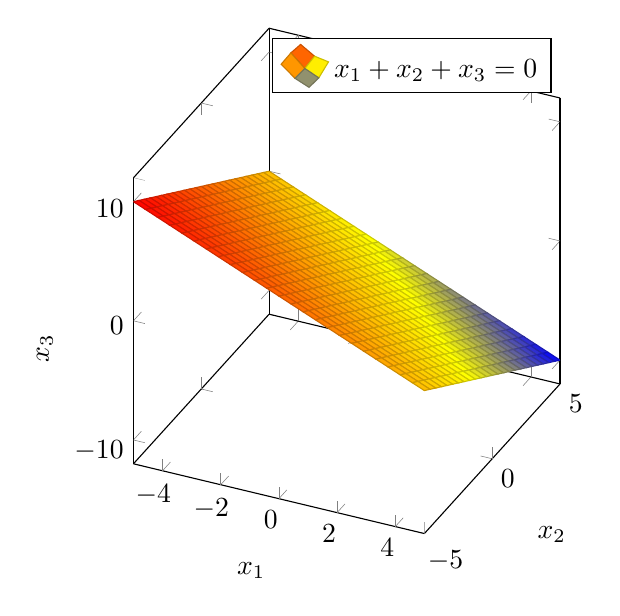
\begin{tikzpicture}
    \begin{axis}[
    width=7cm,height=8cm,
        xlabel = $x_1$,
    ylabel = {$x_2$},
    zlabel = $x_3$]
    \addplot3[
        surf,
    ]
    {-(x+y)};
    \addlegendentry{$x_1 + x_2 + x_3 = 0$}
    \end{axis}
    \end{tikzpicture}
	
	    \noindent\rule{\textwidth}{1pt}
	    
	\item \points{2} Given some $x_0 \in \R^n$, find the \emph{squared distance} to the hyperplane defined by $w^T x + b=0$.
	In other words, solve the following optimization problem:
	\begin{align*}
	\min_x& \|x_0 - x \|^2\\
	\text{s.t. }&w^Tx +b = 0
	\end{align*}
	(Hint: if $\widetilde{x}_0$ is the minimizer of the above problem, note that $\| x_0 - \widetilde{x}_0 \| = | \frac{w^T(x_0 - \widetilde{x}_0)}{\|w\|} |$. What is $w^T \widetilde{x}_0$?)\\
\\
    \noindent\rule{\textwidth}{1pt}
    {\bf Solution:}\\
    Let $x^*$ be the minimizer of the optimization problem, that is, let $x^*$ be the projection of $x_0$ onto the hyperplane. Then, the distance from $x_0$ to the hyperplane would be given (as the hint states) by the difference of the lengths of the projections of $x_0$ and $x^*$ onto the normal vector $w$:
    $$
    \|x_0 - x^*\| = \left| \frac{w^Tx_0}{\|w\|} - \frac{w^Tx^*}{\|w\|}\right| = \left|\frac{w^T(x_0 - x^*)}{\|w\|} \right|
    $$
    Since $x^*$ lies in the hyperplane, we have $w^Tx^* + b = 0$. Thus:
    $$
    \boxed{
    \|x_0 - x^*\|^2 = \left|\frac{w^Tx_0 + b}{\|w\|} \right|^2
    }
    $$
    \noindent\rule{\textwidth}{1pt}
    
\end{enumerate} 

A.10 For possibly non-symmetric $\mat{A}, \mat{B} \in \R^{n \times n}$ and $c \in \R$, let $f(x, y) = x^T \mat{A} x + y^T \mat{B} x + c$. Define $\nabla_z f(x,y) = \begin{bmatrix} \frac{\partial f(x,y)}{\partial z_1} & \frac{\partial f(x,y)}{\partial z_2} & \dots & \frac{\partial f(x,y)}{\partial z_n} \end{bmatrix}^T$.  
\begin{enumerate}
	\item \points{2} Explicitly write out the function $f(x, y)$ in terms of the components $A_{i,j}$ and $B_{i,j}$ using appropriate summations over the indices.
	\\
\\
    \noindent\rule{\textwidth}{1pt}
    {\bf Solution:}\\
     $$
     \boxed{f(x,y) = \sum_{i=1}^n \sum_{j=1}^n A_{ij}x_i x_j + \sum_{i=1}^n \sum_{j=1}^n y_i B_{ij} x_j + c  }
     $$
     
     
    \noindent\rule{\textwidth}{1pt}
	\item \points{2} What is $\nabla_x f(x,y)$ in terms of the summations over indices \emph{and} vector notation?\\
\\
    \noindent\rule{\textwidth}{1pt}
    {\bf Solution:}\\
    $$
    \boxed{ (\nabla_x f(x,y))_k =  \frac{\partial f(x,y)}{\partial x_k} = \sum_{\substack{j=1\\  j\not=k}}^n A_{kj}x_j + \sum_{\substack{i=1\\  i\not=k}}^n A_{ik}x_i + 2A_{kk}x_k + \sum_{i=1}^n y_iB_{ik} = \sum_{\substack{j=1}}^n A_{kj}x_j + \sum_{\substack{i=1}}^n A_{ik}x_i + \sum_{i=1}^n y_iB_{ik}}
    $$
    Expressing the above in the vector form:
    $$
    \boxed{\nabla_x f(x,y) = (A + A^T)x + B^Ty}
    $$
    \noindent\rule{\textwidth}{1pt}
	\item \points{2} What is $\nabla_y f(x,y)$ in terms of the summations over indices \emph{and} vector notation?
	\\
\\
    \noindent\rule{\textwidth}{1pt}
    {\bf Solution:}\\
    $$
    \boxed{ (\nabla_y f(x,y))_k =  \frac{\partial f(x,y)}{\partial y_k} = \sum_{j=1}^n B_{kj}x_j}
    $$
    Epressing the above in the vector form:
    $$
    \boxed{ \nabla_y f(x,y) =  Bx}
    $$
    \noindent\rule{\textwidth}{1pt}
\end{enumerate}

B.2 \points{1} The \textit{trace} of a matrix is the sum of the diagonal entries; $Tr(A) = \sum_i A_{ii}$. If $A\in\mathbb{R}^{n\times m}$ and $B\in\mathbb{R}^{m\times n}$, show that $Tr(AB) = Tr(BA)$.	\\
\\
    \noindent\rule{\textwidth}{1pt}
    {\bf Solution:}\\
    \begin{itemize}
        \item Note that $(AB)_{ii} = \sum_{j=1}^m A_{ij}B_{ji}, \quad (BA)_{jj} = \sum_{i=1}^n B_{ji}A_{ij}$
        \item Then: 
        $$
        Tr(AB) = \sum_{i=1}^n(AB)_{ii} = \sum_{i=1}^n\sum_{j=1}^m A_{ij}B_{ji} =
        \sum_{j=1}^m\sum_{i=1}^n B_{ji}A_{ij} = \sum_{j=1}^m(BA)_{jj} = Tr(BA) \qquad \Box
        $$
    \end{itemize}        


    \noindent\rule{\textwidth}{1pt}

B.3 \points{1} Let $v_1,\dots,v_n$ be a set of non-zero vectors in $\mathbb{R}^d$. Let $V = [v_1,\dots,v_n]$ be the vectors concatenated. 
    \begin{enumerate}
        \item What is the minimum and maximum rank of $\sum_{i=1}^n v_i v_i^T$?
        \\
        \\
            \noindent\rule{\textwidth}{1pt}
            {\bf Solution:}\\
            Note that $\sum_{i=1}^n v_i v_i^T = VV^T$. Since the $v_i$ are nonzero, the minimum rank cannot be zero (since only zero matrix is of zero rank), so we have:
            $$
            \boxed{ 1 \le \rank VV^T \le \rank V \le \min(n,d)}
            $$
            An example of the minimum rank 1 would be to take $V$ with all the columns equal to the same vector, then both $V$ and $VV^T$ would be rank 1.
            An example of the maximum rank would be
            \begin{itemize}
                \item For $n >= d$: let $V$ be a matrix with $n$ orthonormal columns, then $VV^T$ and $V$ would be full rank.
                \item For $d >= n$: let $V$ be a matrix with $d$ orthonormal rows, then $VV^T$ and $V$ would be full rank.
            \end{itemize}
            (In fact, it can be shown that $\rank VV^T = \rank V$ by taking the reduced SVD of V and obtaining the SVD of $VV^T$ with the same number of nonzero singular values which is equal to rank.
            $$
            V = \hat U \hat \Sigma \hat V^T \Rightarrow VV^T = \hat U \hat \Sigma \hat V^T \hat V \hat \Sigma \hat U^T = \hat U \hat \Sigma^2 \hat U^T
            $$
            Now, $\hat \Sigma$ and $\hat \Sigma^2$ have the same number of nonzero elements, so $\rank VV^T = \rank V \qquad \Box$)
            
            \noindent\rule{\textwidth}{1pt}
        \item What is the minimum and maximum rank of $V$?
        \\
        \\
            \noindent\rule{\textwidth}{1pt}
            {\bf Solution:}\\
            Again, since $v_i$ are nonzero, we cannot have zero rank. The full rank would be $\min(d,n)$ (by definition). Examples are given in a.
            $$ 
            \boxed{1 \le \rank V \le \min(d,n)}
            $$
        
            \noindent\rule{\textwidth}{1pt}
        \item Let $A \in \mathbb{R}^{D \times d}$ for $D > d$. What is the minimum and maximum rank of $\sum_{i=1}^n (A v_i) (A v_i)^T$?
        \\
        \\
            \noindent\rule{\textwidth}{1pt}
            {\bf Solution:}\\
            Note that $\sum_{i=1}^n (A v_i) (A v_i)^T = (AV)(AV)^T$. Then, since $D>d$:
            $$
            \boxed{ 0 \le \rank(AV)(AV)^T \le \rank(AV) \le \min(\rank A, \rank V) \le \min(n,d)}
            $$
            For rank 0 take zero $A$, for rank $\min(n,d)$ take full-rank $V$ and full-rank $A$ (because in the latter case $AV$ is full rank and so is $(AV)(AV)^T$ by a.).
        
            \noindent\rule{\textwidth}{1pt}
        \item What is the minimum and maximum rank of $AV$? What if $V$ is rank $d$?
        \\
        \\
            \noindent\rule{\textwidth}{1pt}
            {\bf Solution:}\\
            \begin{itemize}
            \item
            $$
            \boxed{ 0 \le \rank(AV) \le \min(\rank A, \rank V) \le \min(n,d)}
            $$
            For rank 0 take zero $A$, for rank $\min(n,d)$ take full-rank $V$ and full-rank $A$ (so that $AV$ is full-rank).
            \item $V$ of rank $d$ implies $n>=d$ and thus (since $D>d$):
            $$
            \boxed{ 0 \le \rank(AV) \le \min(\rank A, \rank V) \le d}
            $$
            \end{itemize}
        
            \noindent\rule{\textwidth}{1pt}
    \end{enumerate}

\subsection*{Programming}

A.11 For the $A, b, c$ as defined in Problem 8, use
  NumPy to compute (take a screen shot of your answer):
  \begin{enumerate}
  \item \points{2} What is $A^{-1}$?
  \item \points{1} What is $A^{-1}b$? What is $Ac$?
  \end{enumerate}\\
        \\
            \noindent\rule{\textwidth}{1pt}
            {\bf Solution:}\\  
            See Figure 1.
            \begin{figure}[h!]
            \centering
            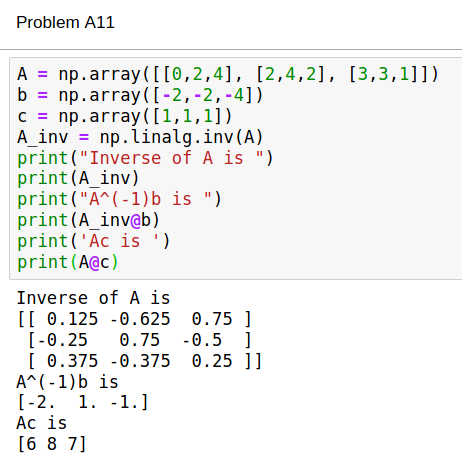
\includegraphics[width=0.33\textwidth]{A11.png}
            \caption{Screenshot of the solution for A11}
            \end{figure}
\begin{python}
#Code for A11
import numpy as np
A = np.array([[0,2,4], [2,4,2], [3,3,1]])
b = np.array([-2,-2,-4])
c = np.array([1,1,1])
A_inv = np.linalg.inv(A)
print("Inverse of A is ")
print(A_inv)
print("A^(-1)b is ")
print(A_inv@b)
print('Ac is ')
print(A@c)
\end{python}
\noindent\rule{\textwidth}{1pt}
A.12 \points{4} Two random variables $X$ and $Y$ have equal
  distributions if their CDFs, $F_X$ and $F_Y$, respectively, are
  equal, i.e. for all $x$, $ |F_X(x) - F_Y(x)| = 0$. 
The central limit theorem says that the sum of $k$ independent,
zero-mean, variance-$1/k$ random variables converges to a (standard) Normal distribution as $k$ goes off to infinity.  
We will study this phenomenon empirically (you will use the Python packages Numpy and Matplotlib). 
Define $Y^{(k)} = \frac{1}{\sqrt{k}} \sum_{i=1}^k B_i$ where each $B_i$ is equal to $-1$ and $1$ with equal probability.
From your solution to problem 5, we know that $\frac{1}{\sqrt{k}} B_i$ is zero-mean and has variance $1/k$.
\begin{enumerate}
\item For $i=1,\dots,n$ let $Z_i \sim \mathcal{N}(0,1)$. If
  $F(x)$ is the true CDF from which each $Z_i$ is drawn (i.e.,
  Gaussian) and $\widehat{F}_n(x) = \frac{1}{n} \sum_{i=1}^n
  \1\{ Z_i \leq x)$, use the answer to problem 1.5  above to choose
  $n$ large enough such that, for all $x \in \R$, $ \sqrt{\E[
    (\widehat{F}_n(x)-F(x))^2 ]} \leq 0.0025$, and plot
  $\widehat{F}_n(x)$ from $-3$ to $3$. \\(Hint: use
  \texttt{Z=numpy.random.randn(n)} to generate the random
  variables, and \texttt{import matplotlib.pyplot as plt};\\
  \texttt{plt.step(sorted(Z), np.arange(1,n+1)/float(n))} to
  plot). 
\item For each $k \in \{1, 8, 64, 512\}$ generate $n$
  independent copies $Y^{(k)}$ and plot their empirical CDF on
  the same plot as part a.\\ (Hint: 
  $\texttt{np.sum(np.sign(np.random.randn(n,
    k))*np.sqrt(1./k), axis=1)}$ generates $n$ of the
  $Y^{(k)}$ random variables.) 
\end{enumerate}
Be sure to always label your axes. 
Your plot should look something like the following (Tip: checkout \texttt{seaborn} for instantly better looking plots.)

\begin{center}
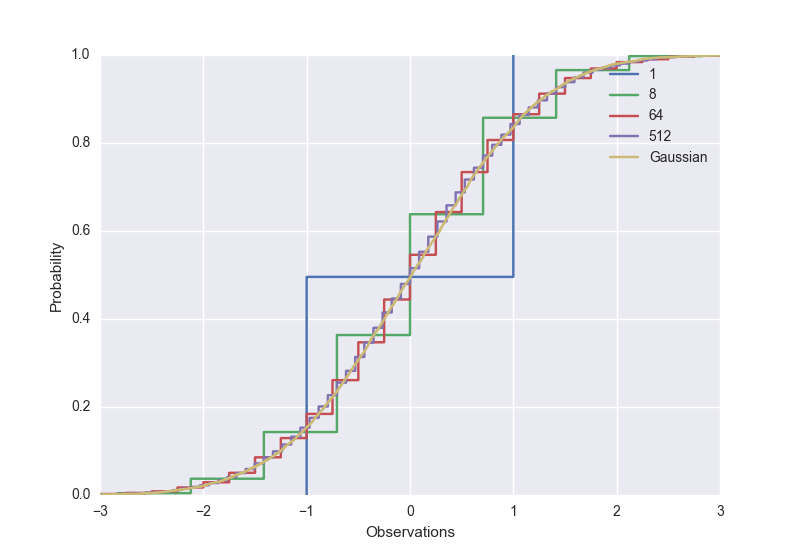
\includegraphics[width=4in]{full.png}
\end{center} 

\\
        \\
\noindent\rule{\textwidth}{1pt}
{\bf Solution:}\\
a. See Figure 2 for the plot of empirical CDF of the standard normal.
Using the $\frac{1}{4n}$ bound in A.6, we find that $n = 40000$ is sufficient to guarantee the required error from the true CDF.

\begin{figure}[h!]
\centering
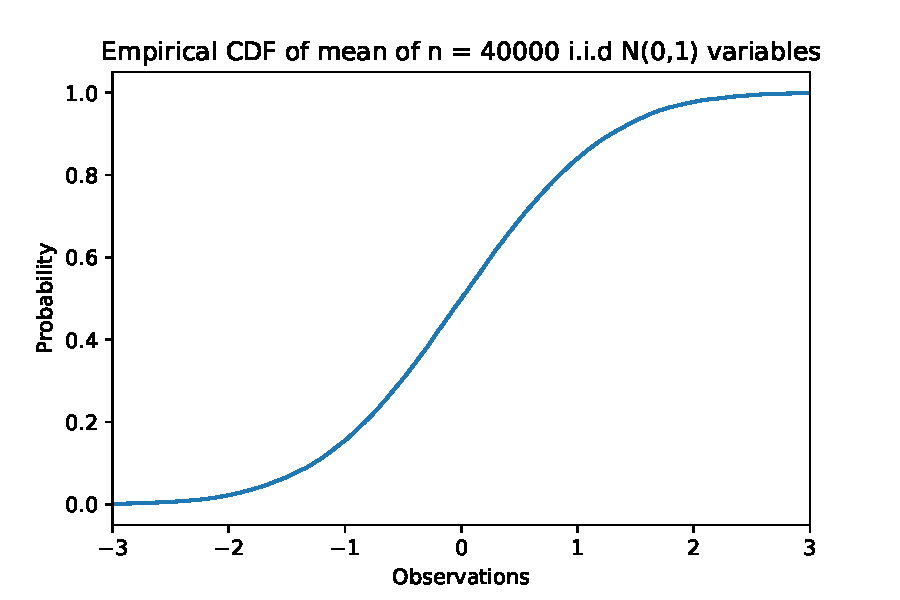
\includegraphics[width=0.6\textwidth]{A12a_CDF.pdf}
\caption{Empirical CDF for A12a}
\end{figure}


\begin{python}
#Code for A12.a
import numpy as np
import matplotlib.pyplot as plt
n = 40000
Z = np.random.randn(n)
ax = plt.gca()
plt.step(sorted(Z), np.arange(1,n+1)/float(n))
plt.title("Empirical CDF of mean of n = 40000 i.i.d N(0,1) variables")
ax.set_xlim((-3,3))
plt.xlabel('Observations')
plt.ylabel('Probability')
plt.savefig('A12a_CDF.pdf')
\end{python}

\\
b. See Figure 3.
\begin{figure}[h!]
\centering
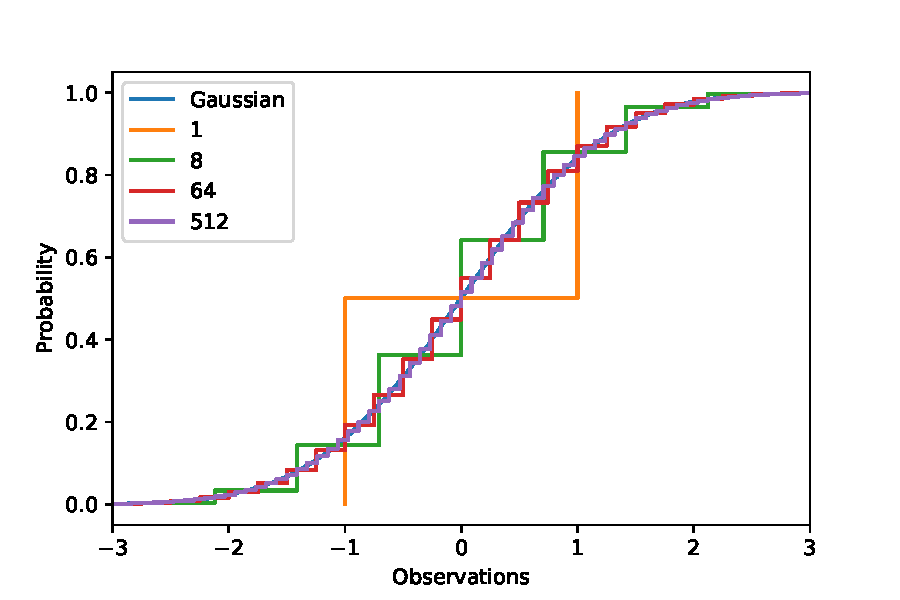
\includegraphics[width=0.6\textwidth]{A12b.pdf}
\caption{A12b}
\end{figure}
\newpage
\begin{python}
#Code for A12.b
import numpy as np
import matplotlib.pyplot as plt
n = 40000
Z = np.random.randn(n)
ax = plt.gca()
plt.step(sorted(Z), np.arange(1,n+1)/float(n), label = 'Gaussian')

for k in [1,8,64,512]:
    Z_k = np.sum(np.sign(np.random.randn(n, k))*np.sqrt(1./k), axis=1) 
    plt.step(sorted(Z_k), np.arange(1,n+1)/float(n), label='%s' % k)

ax.set_xlim((-3,3))
plt.legend()
plt.xlabel('Observations')
plt.ylabel('Probability')
plt.savefig('A12b.pdf')
\end{python}
\noindent\rule{\textwidth}{1pt}
            


\end{document}
